\subsection{Spherical Grains}
In Table \ref{tab:dust_model_fits_spherical} we report the scale factor, chi-squared and maximum dust grain size for 4 values of posisity, with multiple fit types. 


We can see that across all of the fits, the best fit (lowest chi-squared) is the fit with a porosity of $f$ = 0.75 when we include all bands. However, we also note that the results comparing all bands versus Band 5 not included are essentially the exact same. 

In Figure \ref{fig: DustModels_Spherical_WithoutBand5}, we show the jplots associated with the fit without Band 5. The equivalent plots for the other fits can be found in Appendix \ref{chap: Appendix_DustModels}. In this figure, the observed \POLF value for each band is plotted as a colour-matching marker, the values of these are listed in Table \ref{tab:polf_comparison}, in the POLF$_{\text{max \SI}}$ column. 

This figure highlights how the Band 5 marker (yellow triangle) is significantly lower than the model predicts. However, the robust = -1 Band 5 marker (green plus sign)is a much better match. 

\begin{table}[h!]
\centering
\caption{\note{This was last updated on May 6th. Also ensure consistent precision across all entries.}}
\begin{tabular}{ccccc}
\toprule
\textbf{Fit Case} & \textbf{Porosity ($f$)} & \textbf{Scale Factor} & $\boldsymbol{\chi^2}$ & $\boldsymbol{\amaxeq}$ (\micron) \\
\midrule

\textbf{All bands} 
& 1.00 & 1.69 & 0.0021 & 165 \\
& 0.75 & 1.60 & 0.0003 & 280 \\
& 0.50 & 1.54 & 0.0021 & 535 \\
& 0.25 & 1.51 & 0.0160 & 1724 \\

\midrule

\textbf{No Band 5} 
& 1.00 & 1.69 & 0.0020 & 165 \\
& 0.75 & 1.60 & 0.0005 & 280 \\
& 0.50 & 1.53 & 0.0022 & 535 \\
& 0.25 & 1.50 & 0.0160 & 1724 \\

\midrule

\textbf{No Band 6} 
& 1.00 & 1.69 & 0.0020 & 165 \\
& 0.75 & 1.59 & 0.0003 & 280 \\
& 0.50 & 1.53 & 0.0022 & 535 \\
& 0.25 & 1.48 & 0.0263 & 1851 \\

\midrule

\textbf{Bands 4 \& 7} 
& 1.00 & 1.74 & 0.0058 & 166 \\
& 0.75 & 1.58 & 0.0009 & 277 \\
& 0.50 & 1.52 & 0.0034 & 535 \\
& 0.25 & 1.47 & 0.0959 & 2234 \\

\bottomrule
\end{tabular}
\label{tab:dust_model_fits_spherical}
\end{table}






\begin{figure*}[h]
  \centering
  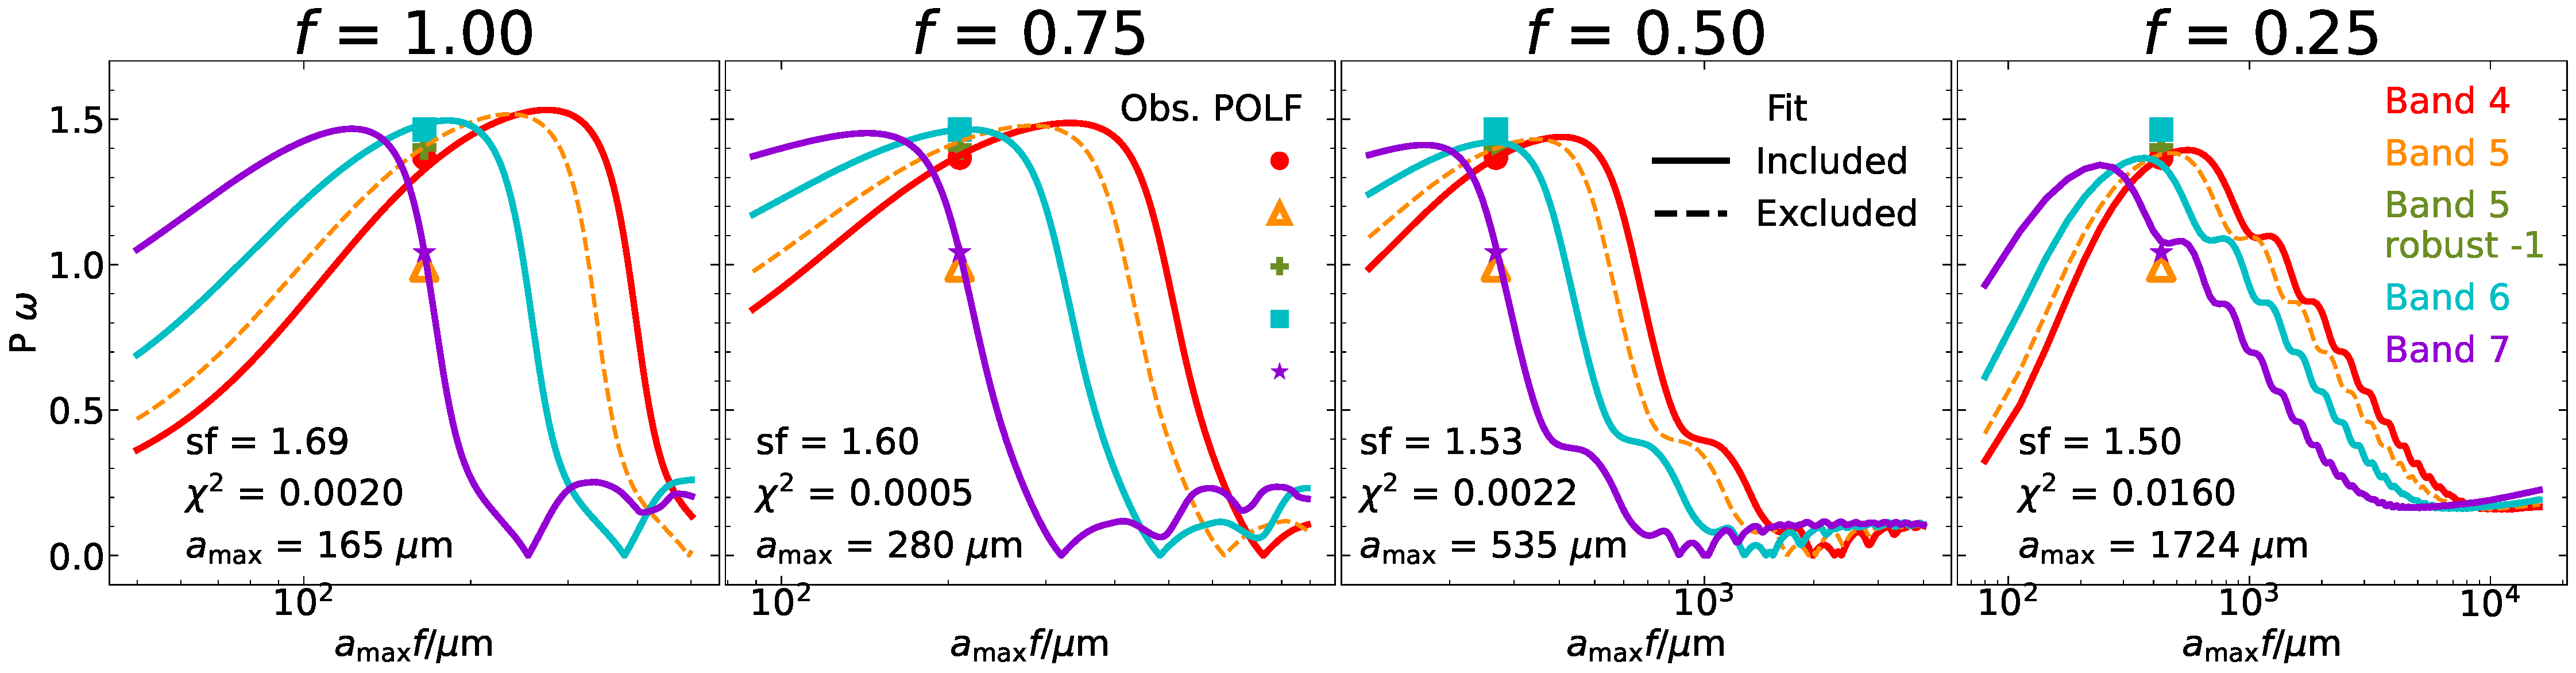
\includegraphics[width=1.1\textwidth]{WRITEUP_AND_IMAGES/IMAGES/WRITEUP/DustModels/DustModelPlot_Without5.pdf}
  \caption{\add{caption}}
  \label{fig: DustModels_Spherical_WithoutBand5}
\end{figure*}


% ----------------------------------------------
\subsection{Non-Spherical Grains}